
% This LaTeX was auto-generated from MATLAB code.
% To make changes, update the MATLAB code and republish this document.

\documentclass{article}
\usepackage{graphicx}
\usepackage{color}

\sloppy
\definecolor{lightgray}{gray}{0.5}
\setlength{\parindent}{0pt}

\begin{document}

    
    
\section*{Task 2}

\begin{par}
Analysis of piloted airplaine stability.
\end{par} \vspace{1em}

\subsection*{Contents}

\begin{itemize}
\setlength{\itemsep}{-1ex}
   \item Transfer function
   \item Step response and stability
   \item Propotional control transfer function
   \item P-control stability
   \item Kp-stable values
   \item Control system step response
   \item Simulink step response
\end{itemize}


\subsection*{Transfer function}

\begin{par}
the transfer function, with canard deflection as input and pitch altitude as output, is given as:
\end{par} \vspace{1em}
\begin{par}
$$ \frac{\theta}{\delta_c} = \frac{s+24}{(s-8)(s-18)} $$
\end{par} \vspace{1em}
\begin{par}
This system is clearly unstable, as both poles are positive real numbers (8 and 18). We can verify this by using pzplot and looking at the poles:
\end{par} \vspace{1em}
\begin{verbatim}
s = tf('s');
sys = (s+24)/((s-8)*(s-18));
pzplot(sys);
\end{verbatim}

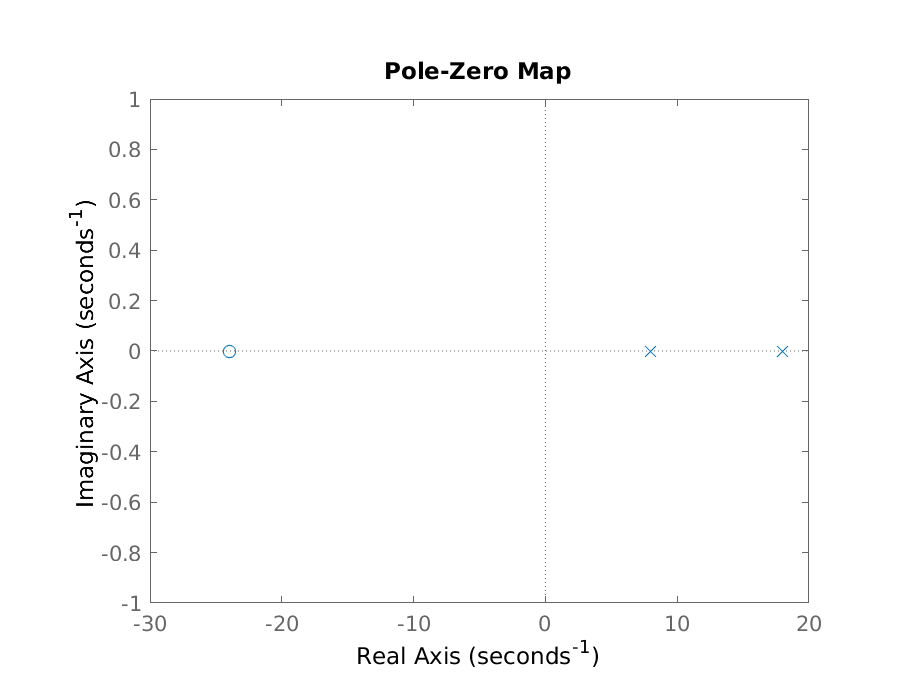
\includegraphics [width=4in]{main_01.eps}
\begin{par}
As we can see, both poles have positive real part, so the system must be unstable
\end{par} \vspace{1em}


\subsection*{Step response and stability}

\begin{verbatim}
close;
step(sys);
\end{verbatim}

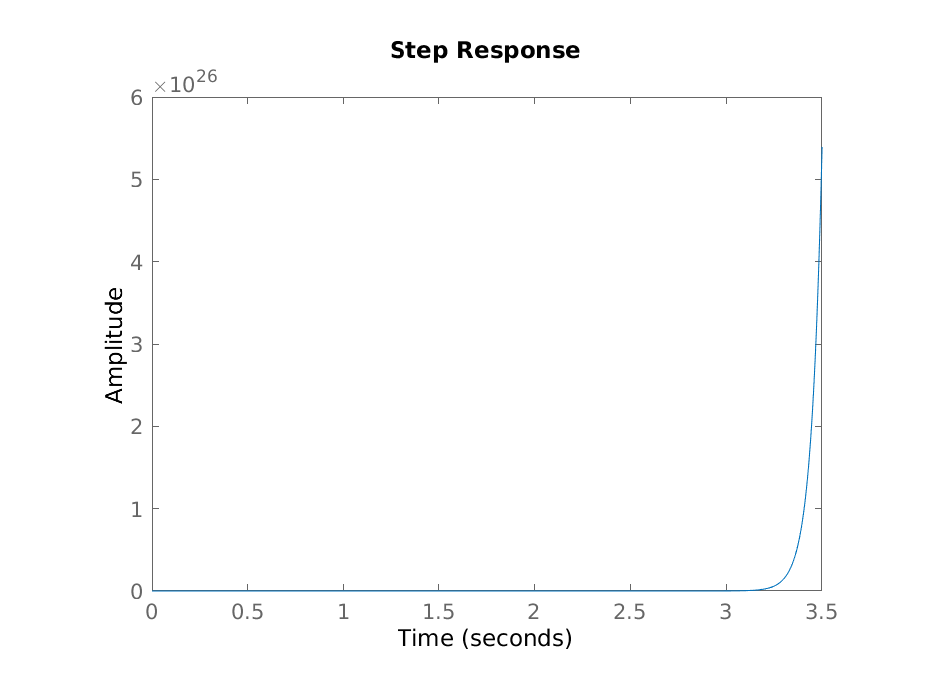
\includegraphics [width=4in]{main_02.eps}
\begin{par}
The output of our system blows up to infinity, so it is clearly unstable.
\end{par} \vspace{1em}
\begin{par}
The open-loop system does not satisfy BIBO, and requires closed loop control to become stable.
\end{par} \vspace{1em}


\subsection*{Propotional control transfer function}

\begin{par}
We add a proportional control and find an equivalent transfer function for the whole system. I use the simulink block diagram to help find the expression for the new system.
\end{par} \vspace{1em}
\begin{par}
$$ \theta = K_p \theta_c H(s) - K_p\theta H(s)$$
\end{par} \vspace{1em}
\begin{par}
$$\theta(K_p H(s) + 1) = \theta_c K_p H(s)$$
\end{par} \vspace{1em}
\begin{par}
$$\frac{\theta}{\theta_c} = \frac{K_p H(s)}{K_p H(s) + 1}$$
\end{par} \vspace{1em}
\begin{par}
I insert the plant model $H(s)$ to obtain the full closed loop transfer function:
\end{par} \vspace{1em}
\begin{par}
$$\frac{\theta}{\theta_c} = \frac{K_p \frac{s+24}{s^2-26+144}}{K_p \frac{s+24}{s^2-26+144} + 1} $$
\end{par} \vspace{1em}
\begin{par}
Finally, simplifying the fraction gives:
\end{par} \vspace{1em}
\begin{par}
$$\frac{\theta}{\theta_c} = \frac{K_p s+ K_p 24}{s^2+(K_p-26)s+(144+24K_p)} $$
\end{par} \vspace{1em}
\begin{par}
Now that we have obtained the transfer function for our controlled system, We can plot the step responses for varying Kp's (proportional gains):
\end{par} \vspace{1em}
\begin{verbatim}
figure;
hold on;
for Kp = [50 110 170 200]
    closed_loop = (Kp*s+Kp*24)/(s^2+(Kp-26)*s+(144+24*Kp));
    step(closed_loop);
end

title('Step Response with Different Kp');
legend('Kp = 50', 'Kp = 110', 'Kp = 170', 'Kp = 200');
\end{verbatim}

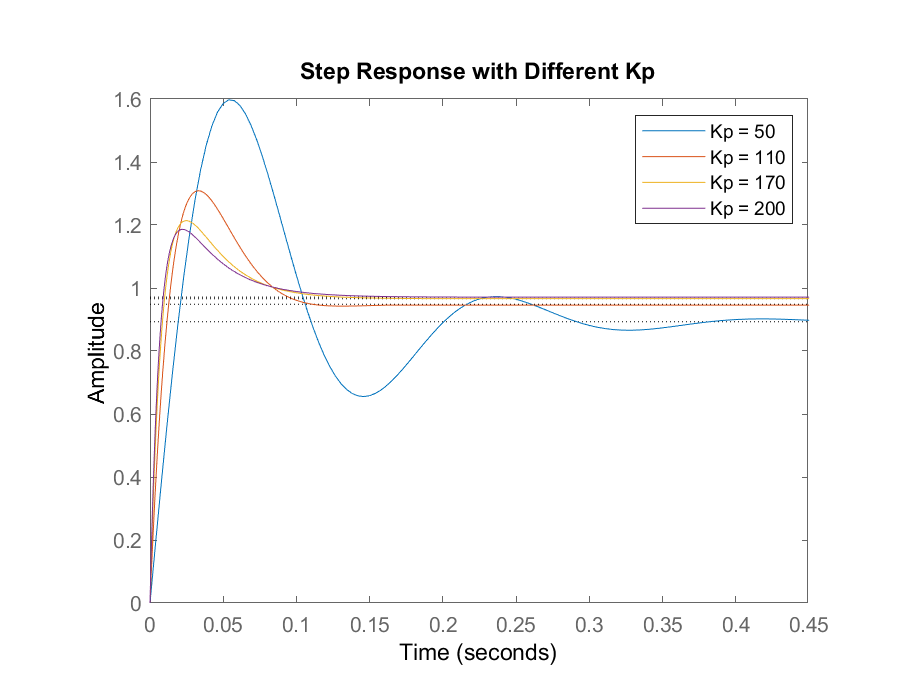
\includegraphics [width=4in]{main_03.eps}
\begin{par}
Increasing the proportional gain results in a shorter rise time, and a smaller steady state error. However, we cannot completely eliminate the steady state error completely, without introducing an integral term.
\end{par} \vspace{1em}


\subsection*{P-control stability}

\begin{par}
We can also plot the poles of this system as a function of the proportional gain $K_p$ The poles are given by the roots of the polynomial in the denominator of our transfer function: We can use the quadratic formula to find the roots and plot $Re\{s\}$ and $Im\{s\}$ separately. We solve the equation:
\end{par} \vspace{1em}
\begin{par}
$$ s^2+(Kp-26)s+(144+24)Kp = 0 $$
\end{par} \vspace{1em}
\begin{verbatim}
close;

Kp = -50:0.05:40; %range of Kp's to analyse
%find poles using the quadratic formula
s_1 = (-(Kp-26)+sqrt((Kp-26).^2-4*(144+24.*Kp)))/2;
s_2 = (-(Kp-26)-sqrt((Kp-26).^2-4*(144+24.*Kp)))/2;

figure;

subplot(2,1,1);
grid on;
hold on;
plot(Kp, real(s_1), 'DisplayName', 'Root 1', 'LineStyle', '-');
plot(Kp, real(s_2), 'DisplayName', 'Root 2', 'LineStyle', '--');
plot(Kp, zeros(size(Kp)), 'k', 'LineWidth', 1);  % x-axis
xlabel('Kp'); ylabel('Real Part of Roots');
title('Real part of poles');
legend;

subplot(2,1,2);
grid on;
hold on;
plot(Kp, imag(s_1), 'DisplayName', 'Root 1', 'LineStyle', '-');
plot(Kp, imag(s_2), 'DisplayName', 'Root 2', 'LineStyle', '--');
plot(Kp, zeros(size(Kp)), 'k', 'LineWidth', 1);  % x-axis
xlabel('Kp'); ylabel('Imaginary Part of Roots');
title('Imaginary part of poles');
legend;
\end{verbatim}

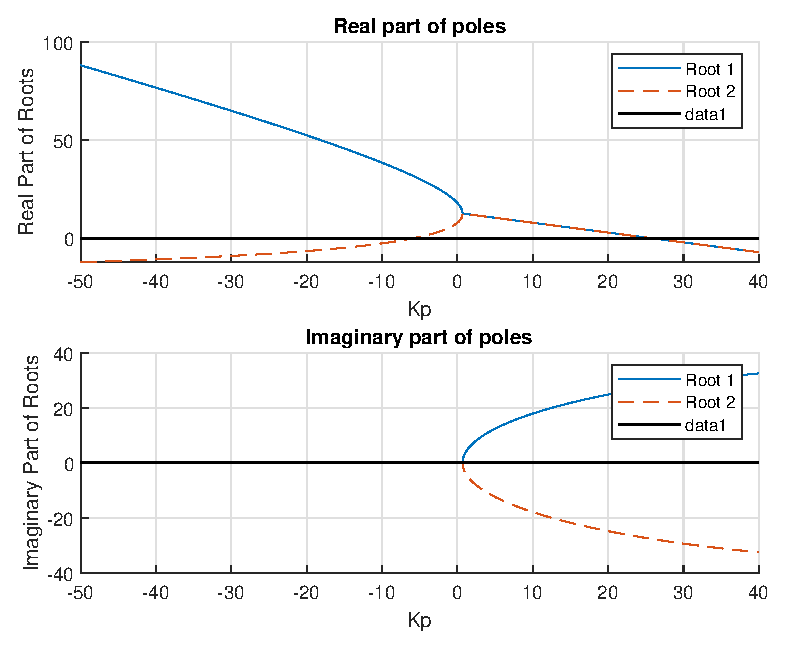
\includegraphics [width=4in]{main_04.eps}


\subsection*{Kp-stable values}

\begin{par}
From inspecting the plot we see that both poles have negative real part when $K_p > 26$.
\end{par} \vspace{1em}
\begin{par}
For the gain, i somewhat arbitrarily chose $Kp = 147.3$, which is where the poles start to separate again:
\end{par} \vspace{1em}
\begin{verbatim}
close;
figure;
grid on;
hold on;

Kp = 144:0.05:150;
s_1 = (-(Kp-26)+sqrt((Kp-26).^2-4*(144+24.*Kp)))/2;
s_2 = (-(Kp-26)-sqrt((Kp-26).^2-4*(144+24.*Kp)))/2;
plot(Kp, real(s_1), 'DisplayName', 'Root 1', 'LineStyle', '-');
plot(Kp, real(s_2), 'DisplayName', 'Root 2', 'LineStyle', '--');

Kp = 147.3;
plot(Kp, (-(Kp-26)+sqrt((Kp-26).^2-4*(144+24.*Kp)))/2, 'marker', '^', 'Color', 'k')
xlabel('Kp'); ylabel('Real Part of Roots');
title('Optimal poles');
legend;
\end{verbatim}

        \color{lightgray} \begin{verbatim}Warning: Imaginary parts of complex X and/or Y arguments ignored. 
\end{verbatim} \color{black}
    
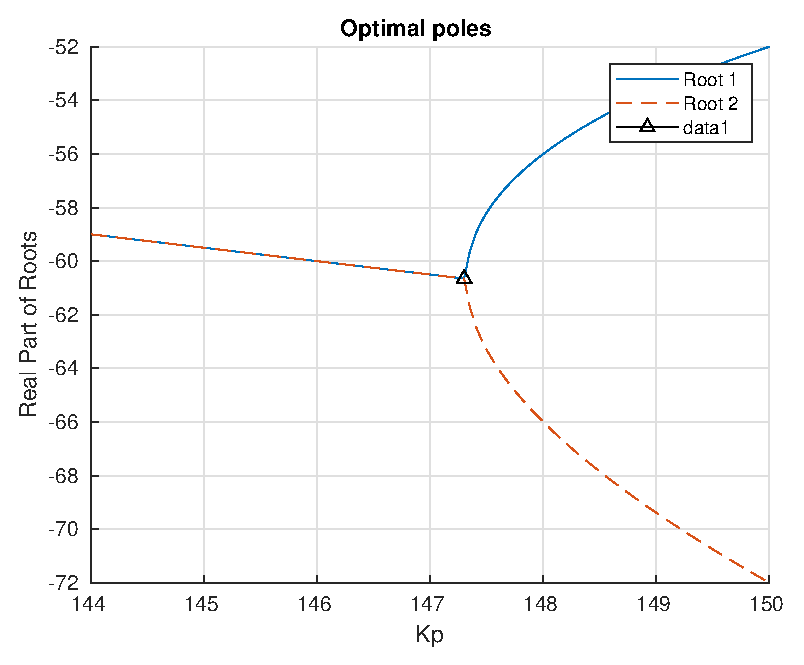
\includegraphics [width=4in]{main_05.eps}
\begin{par}
Verifying that Kp = 26 gives us zero-poles
\end{par} \vspace{1em}
\begin{verbatim}
close;
Kp = 26;
closed_loop = (Kp*s+Kp*24)/(s^2+(Kp-26)*s+(144+24*Kp));
real(pole(closed_loop))
\end{verbatim}

        \color{lightgray} \begin{verbatim}
ans =

     0
     0

\end{verbatim} \color{black}
    \begin{par}
We can check the poles for our new controller with $Kp = 147.3$
\end{par} \vspace{1em}
\begin{verbatim}
Kp = 147;
closed_loop = (Kp*s+Kp*24)/(s^2+(Kp-26)*s+(144+24*Kp));
real(pole(closed_loop))
\end{verbatim}

        \color{lightgray} \begin{verbatim}
ans =

  -60.5000
  -60.5000

\end{verbatim} \color{black}
    \begin{verbatim}
close;
pzplot(closed_loop);
\end{verbatim}

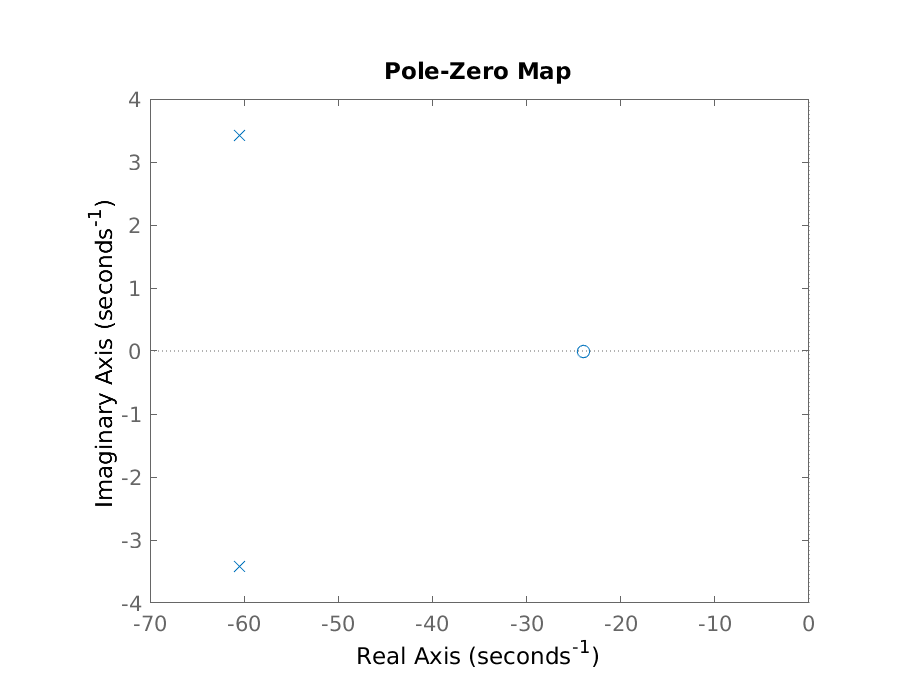
\includegraphics [width=4in]{main_06.eps}


\subsection*{Control system step response}

\begin{par}
We have verified that the poles of our new system are all negative real part. This means the system stable, and we can verify this by viewing the step response of the closed loop system:
\end{par} \vspace{1em}
\begin{verbatim}
step(closed_loop)
[y,t]=step(closed_loop); %save the output values to check steady state
SS_error = abs(1-y(end));
\end{verbatim}

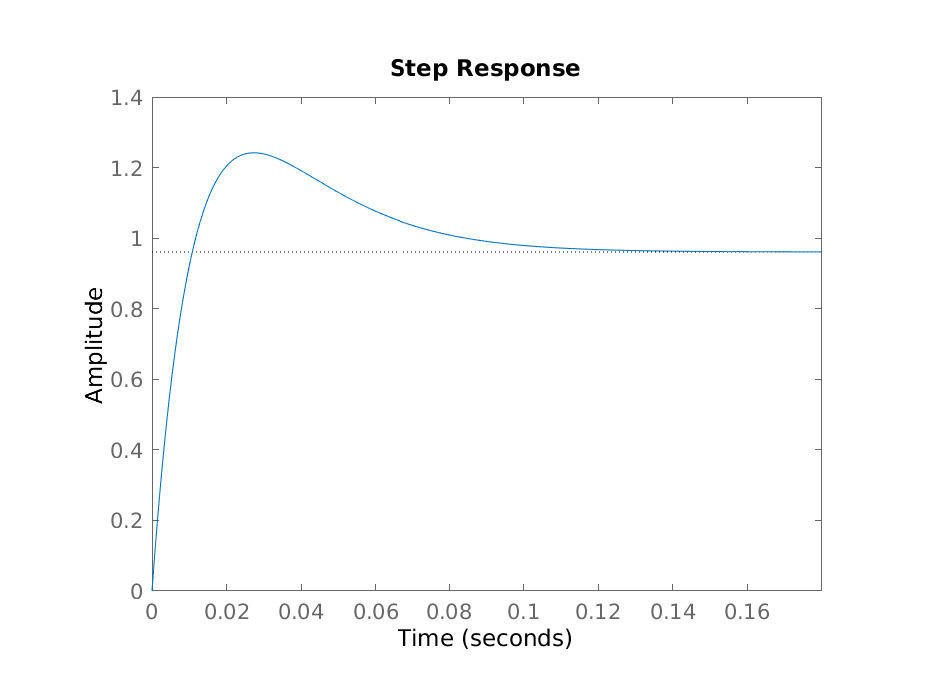
\includegraphics [width=4in]{main_07.eps}
\begin{par}
Thus we have verified that our control system is stable and reaches a steady state error of 3.89\%. We have significant overshoot here, which could be mitigated by incorporating a derivative term (PD control) We can also check that our simulink model agrees with our matlab simulations.
\end{par} \vspace{1em}


\subsection*{Simulink step response}

\begin{par}
Both the original simulink block diagram and the reduced transfer function show the same step response as the matlab code:
\end{par} \vspace{1em}
\begin{par}

\includegraphics [width=4in]{final_step_response.png}

\end{par} \vspace{1em}



\end{document}

